\documentclass[a4paper, openany, 12pt]{article}

%% подключаем стандарт библиографии
\bibliographystyle{gost71u}

%% для "Abstract" в классе book
% \newenvironment{abstract}{}{}
% \usepackage{abstract}

%% подключаем преамбулу: в ней содержится подключение всех необходимых пакетов
%% Работа с русским языком
\usepackage{cmap}			 % поиск в PDF
\usepackage{mathtext} 		 % русские буквы в формулах
\usepackage[T2A]{fontenc}	 % кодировка
\usepackage[utf8]{inputenc}	 % кодировка исходного текста
\usepackage[russian]{babel}	 % локализация и переносы

%% Пакеты для работы с математикой
\usepackage{amsmath,amsfonts,amssymb,amsthm,mathtools}
\usepackage{icomma}

%% Нумерация формул (опционально)
%\mathtoolsset{showonlyrefs=true} % показывать номера только у тех формул, на которые есть \eqref{} в тексте.
%\usepackage{leqno}               % нумерация формул слева

%% Шрифты
\usepackage{euscript}	 % шрифт "Евклид"
\usepackage{mathrsfs}    % красивый мат. шрифт

%% Некоторые полезные макросы для дебага (в случае недоверия авторам шаблона)
\makeatletter
\newcommand\thefontsize{The current font size is: \f@size pt} % пример: \section{\thefontsize}
\makeatother

%% Настройка размеров шрифтов
\makeatletter
\setlength{\headheight}{28pt}
%% TODO: мне не удалось разобраться, как грамотно подбирать второе число в 
%% \@setfontsize\*, но ряд эксппериментов показывает, что "10" выравнивает текст весьма прилично :)
\renewcommand\Huge{\@setfontsize\Huge{14pt}{10}}
\renewcommand\huge{\@setfontsize\huge{14pt}{10}}
\renewcommand\Large{\@setfontsize\Large{14pt}{10}}
\renewcommand\large{\@setfontsize\large{12pt}{10}}
\makeatother

%% Поля (геометрия страницы)
\usepackage[left=3cm,right=1.5cm,top=2cm,bottom=2cm,bindingoffset=0cm]{geometry}

%% Русские списки
\usepackage{enumitem}
\makeatletter
\AddEnumerateCounter{\asbuk}{\russian@alph}{щ}
\makeatother

%% Работа с картинками
\usepackage{caption}
\captionsetup{justification=centering} % центрирование подписей к картинкам
\usepackage{graphicx}                  % вставки рисунков
\graphicspath{{images/}{images2/}}     % папки с картинками
\setlength\fboxsep{3pt}                % отступ рамки \fbox{} от рисунка
\setlength\fboxrule{1pt}               % толщина линий рамки \fbox{}
\usepackage{wrapfig}                   % обтекание рисунков и таблиц текстом

%% Работа с таблицами
\usepackage{array,tabularx,tabulary,booktabs} % дополнительная работа с таблицами
\usepackage{longtable}                        % длинные таблицы
\usepackage{multirow}                         % слияние строк в таблице
\usepackage{makecell}

%% Красная строка
\setlength{\parindent}{2em}

%% Интервалы
\linespread{1}
\usepackage{multirow}

%% TikZ
\usepackage{tikz}
\usetikzlibrary{graphs,graphs.standard}

%% Верхний колонтитул
\usepackage{fancyhdr}
\pagestyle{fancy}

%% Перенос знаков в формулах (по Львовскому)
\newcommand*{\hm}[1]{#1\nobreak\discretionary{}{\hbox{$\mathsurround=0pt #1$}}{}}

%% Дополнительно
\usepackage{float}   % добавляет возможность работы с командой [H] которая улучшает расположение на странице
\usepackage{gensymb} % красивые градусы
\usepackage{caption} % пакет для подписей к рисункам, в частности, для работы caption*
\usepackage{listings} % пакет для листингов с кодом
\lstset{              % настройки для лисингов с кодом
basicstyle=\small\ttfamily,
columns=flexible,
breaklines=true
}

% Hyperref (для ссылок внутри  pdf)
\usepackage[unicode, pdftex]{hyperref}

% Отступ перед первым абзацем в каждом разделе
\usepackage{indentfirst}


\begin{document}
    %% титульник
    % \input{include/title.tex}
    %% аннотоция
    \begin{abstract}

    \begin{center}
        \large{Проектирование системы для потоковой обработки и агрегации данных социальных сетей} \\
    \large\textit{Кидун Станислав Русланович} \\[1 cm]

    Данное исследование направлено на разработку высокопроизводительной системы потоковой обработки данных социальных сетей в реальном времени. Предложена гибридная архитектура, интегрирующая принципы Каппа-архитектуры для устранения дублирования логики и микросервисный подход для обеспечения модульности и горизонтальной масштабируемости. Реализовано решение на базе Apache Kafka (шина событий с "ровно один раз" семантикой) и Apache Flink (движок потоковой обработки), гарантирующее задержку менее 60 секунд от публикации поста в VK до его обработки. Система протестирвоана на основе данных VK. Разработан механизм сбора данных через асинхронный фреймворк vkbottle с динамическим распределением нагрузки по API-токенам, обходящий ограничение на частоту запросов (3 запроса/секунду). Система рассматривает возможности реализации системы хранения данных: Elasticsearch для оперативной аналитики и полнотекстового поиска, Cassandra — для долгосрочного архивирования и интеграции с пакетной обработкой. Практическая проверка подтвердила линейную масштабируемость: обработка 500 сообществ требует 3 токена VK API, 10 000 сообществ — 50 токенов при сохранении целевой задержки. Разработанная платформа имеет практическую значимость для маркетингового анализа трендов, социологических исследований и кризисного мониторинга аномалий, демонстрируя эффективность гибридного подхода для задач Big Data и открывая пути для интеграции новых источников (Telegram, Twitter) и ML-моделей классификации контента.
    \end{center}

\end{abstract}
\newpage
    %% содержание
    \tableofcontents{}
    \newpage

    % \fontsize{14}{16}\selectfont
    \section{Введение}
\label{sec:Chapter0} \index{Chapter0}
    Начало текущего тысячелетия отличилось стремительным развитием цифровых технологий, которые проникли почти во все сферы человеческой деятельности. Одним из ключевых драйверов этого процесса стало повсеместное использование социальных сетей, генерирующих колоссальные объёмы данных в режиме реального времени. Эти данные содержат ценную информацию о поведении пользователей, их предпочтениях и социальных взаимодействиях, что делает их критически важными для бизнеса, маркетинга, социологических исследований и управления общественными процессами. Однако обработка таких данных сопряжена с рядом вызовов, включая необходимость обеспечения высокой производительности, масштабируемости и низкой задержки при анализе потоковой информации.

    \medskip
    Существующие решения для работы с большими данными, такие как пакетная обработка, демонстрируют ограниченную эффективность в контексте динамичных социальных сетей, где задержки в анализе могут привести к утрате актуальности информации. В этой связи особую значимость приобретают системы потоковой обработки, способные агрегировать и анализировать данные в реальном времени. Подобные системы позволяют выявлять тенденции, обнаруживать аномалии и принимать оперативные решения на основе актуальных данных. 

    \subsection{Определения используемые в данной работе}
        Введём несколько определений используемых в данной работе.
        \begin{itemize}
            \item Потоковая обработка данных — это процесс обработки и объединения данных в режиме реального времени по мере их поступления из непрерывных источников.
            \item Пакетная обработка данных — это процесс обработки, где данные накапливаются и анализируются постфактум.
            \item Бэкенд (Backend) — это внутренняя часть программной или информационной системы, которая отвечает за ее функциональность и обработку данных. 
            \item Фронтенд (Frontend) в контексте веб-разработки относится к той части веб-прило-жения, которую видит пользователь и с которой он непосредственно взаимодействует
            \item СУБД — это программа, которая позволяет создавать базы данных и управлять ими. Она обеспечивает надёжное хранение информации, а также её безопасность и целостность. Помимо этого, СУБД предоставляет администратору средства для управления базой данных.
            \item API (Application Programming Interface) — это программный интерфейс, который позволяет одной компьютерной программе взаимодействовать с другими программами. Он предоставляет набор функций, объектов или действий, которые могут быть использованы разработчиками для создания приложений.
            \item IoT Мониторинг (IoT-monitoring, от Internet of Things) — процесс отслеживания, анализа и управления производительностью и здоровьем подключенных устройств в экосистеме Internet of Things. Он обеспечивает бесперебойную работу систем, повышает их эффективность и безопасность, предоставляя данные в режиме реального времени для дальнейшего анализа и упреждения проблем.
            \item JSON (расшифровывается как JavaScript Object Notation) — это облегченный формат для хранения и передачи данных. Он использует человекочитаемый текст для представления объектов данных, состоящих из пар <ИМЯ\_СВОЙСТВА>: <ЗНАЧЕНИЕ> и массивов, что упрощает его понимание и использование в различных языках программирования.
            \item RPC (Remote Procedure Call) —
            \item RDD (Resilient Distributed Datasets)
        \end{itemize}

    \subsection{Актуальность темы}
        В современных условиях социальные сети играют центральную роль в формировании информационной среды. Объёмы и скорость публикации данных в соцмедиа (Twitter, Facebook, VK и др.) растут крайне быстро: пользователи ежесекундно публикуют миллионы публикаций, фотографий и видео. Эти данные крайне ценны для самых разных областей — от маркетинга (анализ потребительских предпочтений и отслеживание репутации брендов) до общественной безопасности (мониторинг чрезвычайных ситуаций, выявление фейковых новостей или экстремистских проявлений). Однако эффективная работа с такими потоками требует специальных архитектур и технологий, способных обрабатывать данные в реальном времени с высокими объёмами и низкими задержками. Дело в том, что информация крайне быстро теряет актуальность, задержка в несколько минут или часов может сделать информацию устаревшей. В условиях постоянного роста объёмов данных традиционные методы пакетной обработки уже не отвечают требованиям времени. Отслеживание в потоковом режиме трендов и тенденций, ключевых событий или настроений аудитории даёт существенное преимущество в принятии решений в сфере маркетинга, в то время как своевременное обнаружение дезинформации может оказать значительное влияниие на общественную информацию. Поэтому возникает необходимость перехода к архитектурам, способным обеспечивать масштабируемость, отказоустойчивость и низкие задержки.
\newpage
 %% Введение
    \section{Постановка задачи}
\label{sec:Chapter1} \index{Chapter1}
    \subsection{Цели работы}
        Цель этого исследования заключается в исследовании методов обработки и агрегации данных, разработке собственной системы, а так же поиска возможностей для оптимизации и улучшения производительности в парадигме работы с данными социальных сетей. 
        В силу больших объёмов данных система должна быть способной обеспечить высокую производительность а так же обладать качествами высоконагруженных систем, таких как отказоустойчивость, высокую скорость отклика и быстрое восстановление после падения. Так же в силу разнообразности соцмедиа и отсутствия единых стандартов взаимодействия с ними, система должна обладать высокой гибкостью, что бы обеспечить возможность другим разработчикам создавать свои собственные модули без необхадимости перерабатывать уже разработанные модули. Так же одним из самых важных аспектов системы должно быть оперативное принятие решений на основе анализа поступающих данных. Итого, финальная модель должна соответствовать следующим критериям:
        \begin{itemize}
            \item \textbf{Масштабируемость.} Количество пользователей соцсетей продолжает расти, и система должна устойчиво работать при увеличении трафика в десятки раз без радикальной переработки инфраструктуры.
            \item \textbf{Отказоустойчивость.} Система должна уметь быстро восстанавливаться после падения, для скорейшего восстановления обработки трафика. 
            \item \textbf{Гибкость разработки. Модульность.} В связи с большим разнообразием социальных сетей и возможным появлением новый в будущем, система должна иметь возможность интеграции модулей работы с ними без кординальной переработки.
            \item \textbf{Гибридность с офлайновой аналитикой.} Компании и исследовательские организации хотят сочетать быструю первичную аналитику с более глубокой офлайновой аналитикой на больших исторических объёмах данных. Правильное проектирование стриминговой системы должно учитывать интеграцию с хранилищами больших данных и системами batch-аналитики.
            \item \textbf{Низкая задержка и высокая скорость отклика.} В рамках социальных сетей данные могут быстро терять актуальность поэтому система должна быстро реагировать на новые данные.
        \end{itemize}

    \subsection{Задачи работы}
        Для достижения поставленной цели были сформулированы следующие задачи:
        \begin{itemize}
            \item Изучить и проанализировать современные технологии и архитектуры потоковой обработки данных. Исследовать возможность их применения для работы с социальными сетями.
            \item Определить основные функциональные и нефункциональные требования к системе с учётом особенностей источников данных и существующих компонентов и решений.
            \item Разработать архитектурное решение, включающее выбор подходящих компонентов для обработки, агрегации и хранения данных.
            \item Реализовать прототип системы на основе выбранных технологий и провести его экспериментальную проверку.
            \item Проанализировать результаты экспериментов и оценить эффективность разработанного решения в соответствии с поставленными требованиями и критериями.
            \item Провести анализ написанной системы на возможности её улучшения и расширения в будущем.
        \end{itemize}

\newpage
 %% Постановка задачи
    \section{Анализ технологий и требований}
\label{sec:Chapter2} \index{Chapter2}
    Идея потоковой обработки больших объёмов данный появилась десяток лет назад и активно развивается с каждым годом. Это мотивирует появление новых технологий, компонентов и архитектур. В этой главе мы рассмотрим самый распространённые и актуальные для исследования технологии.   

    \subsection{Существующие архитектуры}
        С появлением задач потоковой обработки данных стали развиваться архитектуры, специализированные на решении данных задач. Далее рассматриваются самые популярные из них: Lambda-архитектура, Каппа-архитектура и Microservices + Event Sourcing:
        \subsubsection{Lambda-архитектура}
            Lambda-архитектура представляет собой гибридную модель проектирования системы обработки данных, направленную на преодоление фундаментального противоречия между низкой задержкой и высокой точностью. Данная парадигма достигает баланса за счёт декомпозиции вычислительного процесса на два независимых, но синхронизированных слоя: пакетный (batch) и скоростной (speed).
            
            Ядро Lambda-архитектуры базируется на трёх инвариантах:
            \begin{enumerate}
                \item \textbf{Неизменяемость данных (Immutability)} — Все входящие события сохраняются в сыром виде в устойчивом хранилище без модификаций.
                \item \textbf{Принцип пересчёта (Recomputation)} — Любое производное представление генерируется исключительно на основе первичных данных через детерминированные функции.
                \item \textbf{Иерархия точности} — Пакетный слой формирует эталонные результаты на полном историческом срезе, тогда как скоростной слой компенсирует его инерционность приближёнными инкрементальными вычислениями.
            \end{enumerate}
            
            Далее рассмотрим архитектурные компоненты и их взаимодействие:
            \begin{itemize}
                \item \textbf{Пакетный слой (Batch Layer)} функционирует как источник истины (source of truth). Он обрабатывает полный архив неизменяемых данных, используя распределённые вычислительные модели типа MapReduce. Результатом являются предварительно агрегированные представления (batch views), например, суточные статистики пользовательской активности. Эти представления материализуются в высокопроизводительных хранилищах типа колоночных баз данных. Ключевой характеристикой слоя является гарантированная точность, достигаемая за счёт полного пересчёта при изменении алгоритмов.
                \item \textbf{Скоростной слой (Speed Layer)} оперирует исключительно новыми событиями, ещё не учтёнными в batch views. Его задача — минимизировать задержку предоставления актуального состояния. Для этого применяются потоковые движки (Apache Storm, Flink), обрабатывающие данные в режиме реального времени. Результаты фиксируются в отдельном хранилище (real-time views), например, key-value базах. Слой жертвует точностью в пользу скорости: возможны временные расхождения из-за отсутствия исторического контекста.
                \item \textbf{Сервисный слой (Serving Layer)} обеспечивает согласованность данных для потребителей. При выполнении запроса он объединяет результаты batch views и real-time views через операцию слияния. Например, суммарное количество транзакций за текущий день будет вычислено как: 
                \begin{equation}    
                    [result] = [speed\_statistics] + [batch\_statistics]
                \end{equation}
            \end{itemize}
            
            
            Несмотря на концептуальную стройность, Lambda-архитектура сталкивается с существенными проблемами в эксплуатации:
            \begin{itemize}
                \item \textbf{Семантический разрыв (Semantic Gap)} — Дупликация бизнес-логики в batch- и speed-слоях ведёт к рискам несогласованности. Например, оконная агрегация в Spark (batch) и Flink (stream) может давать различные результаты из-за различий в реализации.
                \item \textbf{Эксплуатационная сложность} — Поддержка двух независимых вычислительных кластеров (Hadoop для batch, Storm/Flink для stream) требует значительных ресурсов и координации. Синхронизация форматов данных, версий кода и метаданных становится нетривиальной задачей.
                \item \textbf{Латентность обновления эталонных данных} — Периодичность пересчёта batch views (например, раз в сутки) создаёт окна неактуальности, критичные для приложений реального времени.
                \item \textbf{Избыточность хранения} — Сырые данные дублируются в хранилищах для batch (HDFS) и stream (Kafka), увеличивая затраты.
            \end{itemize}
            
            
            Отраслевая практика показала, что классическая Lambda-архитектура эффективна лишь для узкого класса задач (например, финансовый аудит). В ответ на её недостатки возникли модификации:
            \begin{itemize}
                \item \textbf{Гибридные вычисления (Unified Processing)} — Использование фреймворков типа Apache Beam позволяет выполнять один код в режиме batch и stream, устраняя дублирование логики.
                \item \textbf{Оптимизация через Kappa-принципы} — Исторические данные воспроизводятся из потокового лога (Kafka с долгим хранением), сокращая зависимость от пакетного слоя.
                \item \textbf{Stateful Stream Processing} — Движки вроде Flink минимизируют разрыв между точностью и скоростью за счёт управляемых состояний (managed state) и чекипоинтов.
            \end{itemize}
            
            
            В заключении можно сказать, что Lambda-архитектура остаётся значимой теоретической моделью, иллюстрирующей онтологический конфликт между требованиями к задержке и точности в распределённых системах. Её главное наследие — явное разделение ответственности за консистентность (batch) и оперативность (speed). Однако операционные издержки и развитие потоковых технологий смещают фокус в сторону унифицированных подходов. Современные реализации заимствуют идею иерархии точности, но реализуют её через детерминированную реплей данных и транзакционные обновления состояний, что снижает необходимость в дуализме вычислений. Для новых систем целесообразна оценка компромиссов между чистотой Lambda и прагматикой Каппа-архитектур с учётом специфики предметной области.

        \subsection{Kappa Архитектура}
            Каппа-архитектура возникла как методологический ответ на операционные сложности Lambda-подхода, предлагая принципиально иную философию проектирования. Её ядро составляет концепция единого вычислительного конвейера, где все данные — исторические и реального времени — обрабатываются через единую потоковую модель. Эта парадигма устраняет дуализм вычислений, характерный для Lambda, за счёт абстракции неизменяемого лога событий как универсального источника истины.

            
            Каппа-архитектура базируется на трёх фундаментальных принципах:
            \begin{enumerate}
                \item \textbf{Централизация на потоковом логе} — Все входящие события бессрочно сохраняются в распределённом брокере сообщений (Apache Kafka, Pulsar) с гарантией сохранности и порядковой целостности.
                \item \textbf{Обработка через реплей} — Для пересчёта результатов при изменении логики или восстановлении после сбоев система заново обрабатывает релевантные сегменты лога.
                \item \textbf{Детерминизм вычислений} — Повторный прогон тех же данных через обновлённую логику обязан давать консистентный результат, что обеспечивается неизменяемостью событий и идемпотентностью операторов.
            \end{enumerate}

            
            Рассматривая Каппа-Архитектуру более подробно можно выделить следующие \\структурные компоненты:
            \begin{enumerate}
                \item Неизменяемое хранилище событий выполняет роль первичного источника данных. Брокер сообщений организует события в упорядоченные, секционированные последовательности (топики), где каждая запись снабжается монотонно растущим смещением (offset). Долговременное хранение (ретеншн) обеспечивает доступ к полному историческому архиву — от часов до лет в зависимости от требований.
                \item Единый вычислительный слой заменяет дублирующие batch- и speed-компоненты Lambda. Потоковый движок (Apache Flink, Spark Structured Streaming) потребляет данные непосредственно из лога, применяя пользовательскую логику. Ключевая инновация — поддержка репроцессинга: при необходимости система может перезапустить обработку с произвольной точки смещения, игнорируя текущее состояние. Для управления таким пересчётом используются:
                \begin{itemize}
                    \item \textbf{Точки восстановления (savepoints)} — снапшоты состояния вычислений;
                    \item \textbf{Водяные знаки (watermarks)} — механизмы контроля полноты данных при обработке по времени событий.
                \end{itemize}
                \item Сервисный интерфейс предоставляет результаты через материализованные представления. В отличие от Lambda, здесь отсутствует операция слияния — актуальное состояние генерируется исключительно потоковым конвейером и сохраняется в OLAP-хранилищах (ClickHouse), key-value базах (Redis) или специализированных движках (Apache Pinot).
            \end{enumerate}

            
            Говоря про математическую модель архитектуру стоит выделить процесс обработки данных. Выглядит он следующим образом:
            Результат вычислений $R$ в момент $t$ определяется как функция от полного набора событий $S_{[0,t]}$:
            \begin{equation}
                R(t) = \Phi(S_{[0,t]}, \Omega)
            \end{equation}

            где:
            \begin{itemize}
                \item $\Phi$ — потоковая функция обработки,
                \item $\Omega$ — конфигурация состояния (окна, агрегаторы, UDF).
            \end{itemize}
            При изменении $\Omega$ (например, исправлении алгоритма) результат пересчитывается как 
            \begin{equation}
                R`(t)=\Phi_{new}(S_{[0,t]},\Omega_{new}).  
            \end{equation}

            Несмотря на элегантность подхода, архитектура предъявляет жёсткие требования к инфраструктуре:
            \begin{itemize}
                \item \textbf{Производительность брокера} — Длительный ретеншн требует экстремальной масштабируемости хранилища. Например, топик Kafka с ретеншном 1 год при нагрузке 1 TB/день потребует ~365 TB дискового пространства с учётом репликации.
                \item \textbf{Детерминизм операций} — Некорректная обработка времени событий (временных штампов) или неидемпотентные операции приведут к расхождениям при реплее.
                \item \textbf{Ресурсоёмкость репроцессинга} — Полный пересчёт истории может занимать часы, блокируя ресурсы кластера. Техники инкрементального обновления состояний (например, в Flink) смягчают, но не решают проблему.
                \item \textbf{Сложность отладки} — Анализ причин расхождений между разными версиями $R()$ и $R`()$ требует трассировки событий по всему конвейеру.
            \end{itemize}

            
            В сравнении с Lambda-архитектурой, Каппа-архитектура устраняет три фундаментальных ограничения:
            \begin{enumerate}
                \item \textbf{Ликвидация дублирования логики} — Единый код для всех данных вместо раздельных реализаций под batch/stream.
                \item \textbf{Упрощение инфраструктуры} — Отказ от пакетного кластера (Hadoop/Spark) в пользу единого потокового стека.
                \item \textbf{Гарантия согласованности} — Отсутствие семантического разрыва между "точными" и "приближёнными" представлениями.
            \end{enumerate}

            
            Однако Каппа менее устойчива к ошибкам в проектировании: некорректная водяная метка или потеря состояния при реплее фатальны. Lambda же изолирует риски в speed-слое, сохраняя эталонные данные в batch.

            
            Итого, Каппа-архитектура представляет собой эволюционный шаг в направлении унификации вычислительных моделей. Её главное достижение — доказательство возможности построения консистентных систем реального времени без дуализма вычислений. Хотя операционные требования остаются высокими, развитие управляемых сервисов (Confluent Cloud, Amazon MSK) и стандартизация семантик "ровно один раз" (Kafka Transactions, Flink Checkpoints) снижают барьер внедрения. Для современных разработок Каппа служит предпочтительной основой при условии: долговременной сохраняемости событий в брокере, детерминированности бизнес-логики и готовности к компромиссам в ресурсоёмкости репроцессинга. В контексте научной дискуссии она демонстрирует сдвиг парадигмы: от компромиссов между точностью и скоростью — к их синтезу через иммутабельные данные и реиграцию состояний.

        \subsubsection{Microservices + Event Sourcing}
            Микросервисная архитектура, интегрированная с принципами проектирования, опирающихся на события (Event Sourcing), формирует парадигму, где потоки событий становятся центральной осью координации и сохранения состояния. Данный подход трансформирует традиционные модели взаимодействия сервисов через API в декомпозированную систему асинхронной коммуникации, основанной на неизменяемых фактах.
            
            
            Философия архитектуры базируется на двух взаимодополняющих принципах:
            \begin{enumerate}
                \item \textbf{Проектирование с упором на события (Event Sourcing)} — Состояние системы выводится исключительно из последовательности событий, фиксирующих изменения. В отличие от CRUD-моделей, где актуальное состояние хранится напрямую, здесь реконструкция объекта осуществляется путём применения событий в порядке их возникновения.
                \item \textbf{Декомпозиция на микросервисы} — Каждый сервис инкапсулирует собственную бизнес-логику и данные, взаимодействуя с другими исключительно через события. Это устраняет жесткие зависимости, характерные для монолитных систем.
            \end{enumerate}

            
            Ключевым объектом подобного подхода являются брокеры сообщений (Apache Kaf-ka, RabbitMQ), которые одновременно выступают потоками, связывающими сервисы и журналом команд, гарантирующим сохранность и порядок событий.\\

            \textbf{Механизмы взаимодействия компонентов:}
            
            Генерация событий инициируется командами, поступающими в сервисы через общий шлюз, часто называемый Gateway, или от других сервисов. Например, сервис обработки заказов при подтверждении платежа генерирует событие OrderPaid, которое публикуется в соответствующий топик. Каждое событие обычно содержит:
            \begin{itemize}
                \item Уникальный идентификатор агрегата (например, order\_id)
                \item Таймстамп генерации
                \item Полезную нагрузку в формате, независимом от потребителей
            \end{itemize}

            
            Потребители событий (микросервисы-консьюмеры) подписываются на релевантные топики, обновляя свои локальные состояния или инициируя новые процессы. Сервис аналитики может использовать OrderPaid для расчёта метрик выручки, а сервис доставки — для планирования маршрутов.
            
            
            Однако данный подход имеет ряд вызовов и проблем, которые усложняют работу:
            \begin{itemize}
                \item \textbf{Сложность отслеживания причинности} — В распределённых системах события могут поступать с задержками, нарушая локальный порядок. Механизмы водяных знаков (watermarks) и векторных часов частично решают проблему.
                \item \textbf{Управление схемами данных} — Эволюция форматов событий требует стратегий обратной совместимости (Schema Registry, Avro).
                \item \textbf{Ресурсоёмкость пересчёта состояния} — Длительные цепочки событий замедляют восстановление сервисов после сбоев. Оптимизация через снапшоты (snap-shots) текущих состояний.
                \item \textbf{Отладка распределённых процессов} — Трассировка транзакций, затрагивающих несколько сервисов, требует инструментов вроде OpenTelemetry.
                \item \textbf{Гарантии доставки} — Хотя брокеры типа Kafka обеспечивают "ровно один раз" семантику, идемпотентность обработчиков остаётся ответственностью разработчика.
            \end{itemize}

            
            Паттерн CQRS (Command Query Responsibility Segregation) дополняет модель и решает часть проблем, разделяя операции записи и чтения. Синхронизация между частями в таком подходе обеспечивается асинхронно через поток событий, что устраняет блокировки при высокой нагрузке. В таком подходе модель разделяется на следующие компоненты:
            \begin{enumerate}
                \item \textbf{Командная сторона (Write Model)} — обрабатывает команды, валидирует их и генерирует события.
                \item \textbf{Сторона запросов (Read Model)} — строит материализованные представления из потока событий (например, в Elasticsearch для полнотекстового поиска).
            \end{enumerate}

            
            В сравнении с другими архитектурами, микросервисных подход в связке с проектированием, опирающимся на события, имеет следующие приемущества:
            \begin{itemize}
                \item \textbf{Аудит и воспроизводимость} — Полная история событий позволяет реконструировать состояние системы на любой момент времени.
                \item \textbf{Отказоустойчивость} — Потеря состояния сервиса компенсируется переигранием событий из журнала.
                \item \textbf{Гибкая эволюция} — Добавление новых сервисов не требует изменения существующих: достаточно подписки на релевантные события.
                \item \textbf{Масштабируемость} — Независимое шардирование топиков и консьюмерских групп распределяет нагрузку.
                \item \textbf{Согласованность} — Асинхронная модель гарантирует консистентность без распределённых транзакций.
            \end{itemize}

    \subsection{Системы обработки событий}
        Одними из ключевых технологий в задаче потоковой обработки данных являются системы обработки событий. Они выступают в качестве главных артерий системы и решают задачу общения между различными компонентами систимы, а так же занимаются вопросом перемещения больших объёмов данных. Такие системы чаще всего работают с понятиями "потока" или "очереди", которые является основной сущностью, используемой для передачи данных. Вот самые распространённые из них:
        
        \subsubsection{Apache Kafka}
            Apache Kafka представляет собой распределённую платформу для потоковой передачи и обработки данных, разработанную для обеспечения высокой пропускной способности, минимальных задержек и устойчивости к сбоям. Её архитектура основана на модели публикации-подписки, что позволяет эффективно управлять непрерывными потоками информации между разнородными источниками и приложениями. Ключевой особенностью системы является способность обрабатывать миллионы событий в секунду, сохраняя при этом целостность и порядок данных даже в условиях масштабирования или частичных отказов узлов.
            
            
            Основу Kafka составляют топики — логические каналы, через которые данные распределяются между участниками системы. Каждый топик делится на партиции, обеспечивающие параллелизм обработки: записи в рамках партиции упорядочены, что гарантирует консистентность, а распределение партиций между узлами кластера позволяет балансировать нагрузку. Продюсеры — компоненты, ответственные за публикацию данных в топики — взаимодействуют с брокерами (серверами Kafka), которые сохраняют записи на диск с заданной политикой хранения. Консьюмеры, в свою очередь, извлекают данные из топиков, поддерживая как индивидуальное, так и групповое потребление, что обеспечивает гибкость в распределении задач.
            
             
            Важным аспектом архитектуры Kafka является её отказоустойчивость. Механизм репликации позволяет создавать копии партиций на нескольких брокерах, гарантируя доступность данных при выходе узлов из строя. Для координации метаданных кластера (например, информации о расположении партиций) ранее использовался Apache ZooKeeper, однако современные версии Kafka постепенно внедряют встроенные решения для уменьшения внешних зависимостей.
            
            
            Система поддерживает несколько семантик доставки сообщений:
            \begin{itemize}
                \item \textbf{"максимум один раз"} — данные могут быть потеряны, но не доставлены повторно;
                \item \textbf{"минимум один раз"} — гарантируется минимум одна доставка, что может приводить к дублированию;
                \item \textbf{"ровно один раз"} — исключает как потери, так и повторения, достигая идемпотентности операций.
            \end{itemize}

        \subsubsection{Apache Flink}
            Apache Flink представляет собой высокопроизводительный фреймворк с открытым исходным кодом, ориентированный на обработку потоковых и пакетных данных в гибридном формате. В отличие от систем, разделяющих подходы к работе с потоками и статическими наборами данных, Flink унифицирует эти модели через абстракцию бесконечных потоков, где пакетная обработка рассматривается как частный случай потоковой с фиксированным временным окном. Это позволяет разработчикам создавать гибридные приложения, сочетающие аналитику в реальном времени и исторические вычисления.
            
            
            Ключевой особенностью архитектуры Flink является управление состоянием (state management). Система сохраняет промежуточные результаты обработки событий, обеспечивая консистентность даже при сбоях узлов. Механизм чекпоинтов (checkpoints) периодически фиксирует состояние всех операторов в распределённом хранилище, что гарантирует восстановление данных с точностью до последнего корректного состояния. Для достижения семантики "ровно один раз" Flink использует двухфазный протокол фиксации транзакций, что исключает дублирование или потерю информации — критически важное свойство для финансовых систем или аудита.
            
            
            Одним из преимуществ Flink перед аналогами (например, Apache Spark) является нативная поддержка потоковой обработки. Вместо имитации потоков через микропакеты Flink оперирует непрерывными данными, что снижает задержки и повышает эффективность ресурсов. Архитектура фреймворка включает TaskManager (исполнительные узлы) и JobManager (оркестратор задач), распределяющий операции по кластеру. Для балансировки нагрузки Flink динамически перераспределяет задачи между узлами, используя модель data parallelism.
            
            
            Важным аспектом Flink является работа с временными метками. Система различает:
            \begin{itemize}
                \item \textbf{Event time (временной штамп)} — время генерации события источником
                \item \textbf{Processing time} — момент обработки события фреймворком
                \item \textbf{Ingestion time} — время поступления данных в Flink. Поддержка временных штампов позволяет корректно обрабатывать задержанные или неупорядоченные данные, что актуально для IoT-устройств или глобальных систем с неравномерной задержкой сети.
            \end{itemize}
            
            
            Flink предоставляет богатый набор операторов для трансформации данных:
            \begin{itemize}
                \item \textbf{Оконные функции (tumbling, sliding, session windows)} — группировка событий по временным или количественным критериям;
                \item \textbf{CEP (Complex Event Processing)} — обнаружение паттернов в потоках (например, последовательность действий пользователя);
                \item \textbf{Интеграция с ML-библиотеками} — выполнение прогнозных моделей в реальном времени.
            \end{itemize}

        \subsubsection{RabbitMQ}
            RabbitMQ представляет собой брокер сообщений с открытым исходным кодом, реализующий протокол AMQP (Advanced Message Queuing Protocol). Его основная задача — обеспечить надёжную асинхронную коммуникацию между компонентами распределённых систем, что особенно актуально в микросервисных архитектурах и сценариях, требующих декомпозиции задач. В отличие от систем, ориентированных на потоковую обработку, RabbitMQ фокусируется на гарантированной доставке сообщений, управлении очередями и балансировке нагрузки между потребителями.
            
            
            Архитектурные компоненты системы включают:
            \begin{itemize}
                \item \textbf{Обменники (Exchanges)} — точки входа для сообщений, определяющие правила маршрутизации.
                \item \textbf{Очереди (Queues)} — буферы для хранения сообщений до их обработки потребителями.
                \item \textbf{Привязки (Bindings)} — правила, связывающие обменники с очередями на основе ключей маршрутизации.
            \end{itemize}
            
            
            Сообщения публикуются продюсерами в обменники, которые, используя заданный тип (direct, topic, fanout, headers), определяют, в какие очереди они будут направлены. Например, обменник типа fanout рассылает сообщения во все привязанные очереди, а topic позволяет использовать шаблоны для гибкой фильтрации.
            
            
            Гарантии доставки обеспечиваются механизмами подтверждений (acknowledgments). Потребитель отправляет брокеру подтверждение после успешной обработки сообщения. Если подтверждение не получено (например, из-за сбоя), RabbitMQ повторно ставит сообщение в очередь. Для критически важных задач поддерживается режим persistent messages, при котором данные сохраняются на диск, предотвращая потерю при перезапуске сервера.
            
            
            Кластеризация повышает отказоустойчивость системы. RabbitMQ позволяет объединять узлы в кластеры с общими метаданными (информацией об обменниках, очередях), но данные очередей хранятся локально на каждом узле. Для обеспечения избыточности используется зеркалирование очередей (mirrored queues), при котором сообщения реплицируются между узлами. Это минимизирует риск потери данных при выходе из строя отдельных серверов.
            
            Примеры применения RabbitMQ охватывают широкий спектр задач:
            \begin{itemize}
                \item \textbf{Асинхронная обработка задач} — вынесение ресурсоёмких операций (генерация отчётов, обработка изображений) в фоновый режим.
                \item \textbf{Балансировка нагрузки} — распределение запросов между несколькими экземплярами сервиса через конкурентных потребителей.
                \item \textbf{Интеграция разнородных систем} — обеспечение взаимодействия между legacy-приложениями и современными микросервисами через унифицированный интерфейс обмена сообщениями.
            \end{itemize}
            
            В отличие от систем, оптимизированных для потоковой аналитики (например, Apa-che Kafka), RabbitMQ не предназначен для обработки экстремально высоких объёмов данных в реальном времени. Однако его сила заключается в точном управлении жизненным циклом сообщений, гибкой маршрутизации и поддержке сложных сценариев взаимодействия, таких как RPC или распределённые транзакции.

        \subsubsection{Apache Spark Streaming}
            Apache Spark Streaming представляет собой модуль фреймворка Apache Spark, предназначенный для обработки потоков данных через микропакетную модель (micro-bat-ching). В отличие от систем, ориентированных на непрерывную потоковую обработку (например, Flink), Spark Streaming делит входящий поток на небольшие пакеты фиксированного интервала (от миллисекунд до секунд), обрабатывая их как статические RDD-наборы. Это позволяет использовать единую кодовую базу и API для пакетной и потоковой аналитики, обеспечивая согласованность в гибридных сценариях.
            
            
            Он состоит из следующих архитектурных компонент:
            \begin{itemize}
                \item \textbf{Драйвер} — Оркестрирует задачи, разбивает поток на микропакеты (DStreams) и распределяет их по исполнителям.
                \item \textbf{Исполнители} — Обрабатывают пакеты данных на рабочих узлах кластера.
                \item \textbf{Высокоуровневый API} — Предоставляет абстракцию "бесконечной таблицы"\\ над потоком, позволяя применять SQL-подобные операции и декларативные запросы.
            \end{itemize}
            
            
            Ключевыми особенностями можно выделить:
            \begin{itemize}
                \item \textbf{Гарантии "ровно один раз"} — Достигается через комбинацию чекпоинтов состояния (через HDFS/S3) и атомарной записи результатов (начиная с Structured Streaming).
                \item \textbf{Интеграция с экосистемой Spark} — Поддержка MLlib (машинное обучение в реальном времени), GraphX (графовая обработка) и Spark SQL.
                \item \textbf{Обработка по времени событий} — Возможность агрегации данных по временным окнам с учетом меток генерации события, а не времени поступления.
                \item \textbf{Восстановление через чекпоинты} — Восстановление состояния приложения после сбоя из контрольных точек.
            \end{itemize}
            
            
            В отличие от Apache Flink, использующего нативную потоковую модель, Spark Streaming жертвует сверхнизкой задержкой (типично 0.5–2 секунды) в пользу интеграции с пакетной обработкой Spark и богатой экосистемой. Для сценариев, требующих строгого порядка событий и латенции в миллисекунды, предпочтительнее Flink; для аналитических задач с умеренной задержкой и унифицированной кодобазой — Spark Streaming.

        \subsubsection{Apache Storm}
            Apache Storm представляет собой распределённый, отказоустойчивый движок реального времени (true streaming) для обработки неограниченных потоков данных с экстремально низкой задержкой (миллисекунды). Разработанный в Twitter для анализа твитов в реальном времени, Storm фокусируется на простой, высокопроизводительной доставке и трансформации событий, где порядок обработки каждого сообщения критичен. Его архитектура основана на направленном ациклическом графе (DAG) задач, называемом топологией (topology), которая определяет поток данных и логику обработки.
            
            
            Архитектурные компоненты:
            \begin{itemize}
                \item \textbf{Nimbus} — Центральный координатор (аналог JobManager в Flink), отвечающий за распределение кода топологии по рабочим узлам, планирование задач и мониторинг сбоев. Является "главным" узлом кластера (но без единой точки отказа при использовании HA-режима).
                \item \textbf{Supervisor} — Демон, работающий на каждом рабочем узле кластера. Получает задания от Nimbus, запускает и останавливает рабочие процессы (Worker processes), выделенные под выполнение конкретных задач топологии.
                \item \textbf{Worker process} — JVM-процесс, выполняющий часть топологии. Запускает внутри себя Executor'ы (потоки), которые выполняют Task'и (экземпляры компонентов spout или bolt).
                \item \textbf{Spout} — Источник данных в топологии. Читает данные из внешних систем (Kafka, Kinesis, очереди, сокеты) и испускает кортежи (tuples) в топологию. Отвечает за надёжность: отслеживает обработку испущенных кортежей и повторяет отправку при сбоях (в режимах с гарантиями).
                \item \textbf{Bolt} — Обработчик данных. Принимает кортежи от spout'ов или других bolt'ов, выполняет над ними операции (фильтрация, агрегация, обогащение, запись в БД), и может испускать новые кортежи дальше по топологии. Bolt'ы образуют вычислительные вершины графа.
            \end{itemize}
            
                
            Одной из ключевых особенностей Apache Storm является модель True Streaming обработка событий по одному сразу при их поступлении, в отличие от микропакетных моделей (Spark Streaming). Это обеспечивает минимально возможную задержку. Так же отдельно стоит упомянуть возможноть для горизонтального масштабирования системы: Она легко масштабируется добавлением новых рабочих узлов. Параллелизм spout/bolt настраивается независимо.
            
            
            Apache Storm так же может похвастаться отказоустойчивостью: При падении рабочего узла (Worker) Nimbus перезапускает его задачи на других узлах. При падении самого Nimbus, работающие Supervisor'ы и Worker'ы продолжают функционировать до его восстановления (режим HA требует резервного Nimbus и ZooKeeper).
            
            
            Apache Storm так же поддерживает те же гарантии доставки сообщений, что и Apache Kafka:
            \begin{itemize}
                \item \textbf{"максимум один раз" (По умолчанию)} — Кортежи могут быть потеряны при сбое, но не обработаны повторно (производительность выше).
                \item \textbf{"минимум один раз"} — Гарантирует, что каждый кортеж будет обработан минимум один раз (возможны дубли). Достигается механизмом "acknowledgment" (ACK): spout отслеживает кортежи и переиспускает не подтверждённые в течение таймаута.
                \item \textbf{"ровно один раз" (через Trident)} — Предоставляется высокоуровневой абстракцией Trident. Trident группирует кортежи в мелкие пакеты (микробатчи), использует уникальные ID для отслеживания и обеспечивает идемпотентность операций или транзакционное обновление состояния. Однако это увеличивает задержку и сложность.
            \end{itemize}
            
            Для Apache Storm можно выделить следующие отличия от аналогов:
            \begin{enumerate}
                \item \textbf{Apache Kafka} — Storm является кластерным фреймворком (требует Nimbus/Su-pervisors или YARN/K8s), тогда как Kafka — это легковесная система, интегрируемая почти в любое приложение и используемая для координации и хранения состояния. Kafka Streams проще для Kafka-центричных пайплайнов, но Storm универсальнее для источников, не связанных с Kafka.
                \item \textbf{Apache Flink} — Storm имеет более слабую поддержку управления состоянием (state management) и обработки по времени события (временных штампов) по сравнению с Flink. Trident добавляет состояние и "ровно один раз" семантику, но за счет задержки и усложнения модели программирования. Flink изначально создан для управления состоянием и работы с штампами времени событий. Storm имеет меньшую абстрактную задержку, но Flink часто превосходит его в пропускной способности на сложных состояниях.
                \item \textbf{Apache Spark Streaming} — Storm обеспечивает на порядок меньшую задержку (миллисекунды против секунд), так как обрабатывает события по одному, а не микропакетами. Однако Spark Streaming проще интегрируется с пакетной обработкой Spark и экосистемой (MLlib, SQL) и предоставляет более сильные гарантии состояния и временных штампов "из коробки" через Structured Streaming.
            \end{enumerate}

            
            Storm остаётся эффективным выбором для задач, требующих минимально возможной задержки реакции на событие (например, мониторинг сетевой безопасности, простые фильтрации/обогащения в реальном времени, триггеры мгновенных реакций) и где сложное состояние или обработка по временным штампам не являются основным требованием. Его относительная простота также может быть преимуществом для конкретных сценариев. Однако для сложной аналитики с окнами, точным временем событий и богатым состоянием Flink или Spark Structured Streaming часто предпочтительнее.
\newpage
 %% Обзор существующих решений
    \section{Определение требований и компонентов}
\label{sec:Chapter3} \index{Chapter3}
    На основе проведённого анализа существущих технологий и архитектур, к системе были вынесены следующие функциональные и нефункциональные требования:
    \subsection{Требования к системе}
        \subsubsection{Функциональные требования}
            Система должна обеспечивать выполнение следующих функциональных задач:
            \begin{enumerate}
                \item Система обеспечивает непрерывный прием данных, генерируемых пользователями. В качестве источника используются сообщества социальной сети ВКонтанте (VK) 
                \item Система обеспечивает обработку каждого поста (сообщения) с задержкой, не превышающей установленный порог (менее 60 секунд) от момента публикации в VK до завершения его обработки в рамках основного конвейера.
                \item Система обеспечивает асинхронную, надежную и упорядоченную (в рамках партиций) передачу данных между микросервисами, ответственными за различные этапы обработки. Маршрутизация осуществляется через систему обработки событий, выступающую в качестве шины событий. Планируется использование Apache Kafka.
                \item Система обеспечивает сохранение результатов обработки каждого поста в промежуточном хранилище с возможностью последующего извлечения для дальнейшего анализа и агрегации. Данные сохраняются в структурированном виде, пригодном для эффективного выполнения аналитических запросов.
                \item Система обеспечит эффективный полнотекстовый поиск и сложный аналитический запрос по историческим данным, накопленным в результате работы. Планируется использование Elasticsearch для поиска и, возможно, Cassandra (или аналогичной распределенной NoSQL БД) для хранения детализированных данных, оптимизированных под высокую скорость записи и масштабируемость.
            \end{enumerate}

        \subsubsection{Нефункциональные требования}
            Система должна обладать следующими качественными характеристиками:
            \begin{enumerate}
                \item Система гарантирует обработку более 90\% поступающих постов с задержкой менее 60 секунд от момента появления поста в VK до завершения его базовой обработки (FR2). Это требование является основным критерием "реального времени" в рамках данной работы. Система также должна обеспечивать пропускную способность, достаточную для обработки пиковой нагрузки, характерной для выбранных для мониторинга популярных пабликов VK.
                \item Система проектируется с расчетом на горизонтальную масштабируемость. Увеличение объема обрабатываемых данных (числа отслеживаемых пабликов/постов) должно достигаться преимущественно за счет добавления вычислительных ресурсов (нод) и параллельных экземпляров микросервисов без изменения архитектуры. Компаненты системы должны уметь масштабироваться независимо друг от друга.
                \item Система проектируется с расчётом на удобство интеграций сторонних сервисов и добавления нового функционала. Нарпимер добавление новой социальной сети к обработке, нового типа данных, внедрение машинного обучения или добавление новых сообществ и целей к обработке.
            \end{enumerate}

    \subsection{Выбор компонентов}
        \subsubsection{Выбор языка программирования}
            При проектировании системы потоковой обработки данных социальных сетей одним из аспектов является выбор языка программирования, способного обеспечить баланс между производительностью, гибкостью интеграции и скоростью разработки. В качестве потенциальных кандидатов рассматриваются языки с различными парадигмами, включая C++, Java, Go и Python. Каждый из них обладает уникальными характеристиками, однако окончательный выбор должен учитывать специфику задач, связанных с агрегацией данных, взаимодействием с внешними API (например, VK API) и интеграцией с распределёнными системами (Apache Kafka, Flink). Исходя из этих критериев был выбран Python. \\

            \textbf{Критерии выбора}
            \begin{enumerate}
                \item \textbf{Интеграционная гибкость} — поддержка библиотек для работы с разнородными сервисами и протоколами.
                \item \textbf{Скорость разработки} — лаконичность синтаксиса и доступность инструментов для быстрого прототипирования.
                \item \textbf{Производительность} — эффективность выполнения ресурсоёмких операций, таких как обработка потоков данных.
                \item \textbf{Экосистема} — наличие готовых решений для машинного обучения, многопоточности, визуализации, интеграции распределённых систем и работы с Big Data.
            \end{enumerate}
            
            Paссмотрим альтернативы и варианты. В качестве возможных языков были выбраны следующие: \textbf{C++}, \textbf{Java}, \textbf{Go}, \textbf{Python}. Проанализируем их сильные и слабые стороны с учётом заданных критериев. \\

            \textbf{Анализ альтернатив}
            \begin{enumerate}
                \item \textbf{C++} демонстрирует высокую производительность за счёт низкоуровневого управления памятью и оптимизированной компиляции. Это делает его предпочтительным для задач, требующих минимальных задержек. Однако для интеграции с современными облачными сервисами и RESTful API необходима разработка дополнительных обёрток, что увеличивает сроки реализации. Кроме того, отсутствие встроенной поддержки асинхронных операций усложняет работу с потоковыми данными.
                \item \textbf{Java} предлагает развитую экосистему (Spring, Apache Camel) и высокую портируемость за счёт JVM. Тем не менее, строгая статическая типизация и объёмный boilerplate-код замедляют итеративную разработку, что критично для динамично меняющихся требований социальных сетей.
                \item \textbf{Go} выделяется простотой создания многопоточных приложений, но ограниченная поддержка библиотек для интеграции с NLP-фреймворками или аналитическими инструментами снижает его применимость в данном контексте.
                \item \textbf{Python} предлагает высокую скорость разработки за счёт простоты языка и наличия большого числа готовых решений из различных отраслей. Так же Python предлагает широкий выбор специализированных библиотек, для интеграции разнородных сервисов. 
            \end{enumerate}
            
            \textbf{Обоснование выбора: Python} 

            Выбор Python в качестве основного языка для реализации платформы обусловлен необходимостью быстрой интеграции с разнородными сервисами, доступностью специализированных библиотек и снижением временных затрат на разработку. Несмотря на компромиссы в производительности, его экосистема предоставляет инструменты для построения масштабируемых и maintainable-решений, соответствующих требованиям современных социальных медиа. \\

            Python, несмотря на более низкую производительность в сравнении с компилируемыми языками, становится оптимальным решением благодаря следующим факторам:
            \begin{enumerate}
                \item \textbf{Богатая экосистема библиотек:}
                \begin{itemize}
                    \item \textbf{Интеграция с API} — Библиотеки requests, aiohttp, vkbottle и vk-api упрощают взаимодействие с социальными сетями (VK, Telegram) и внешними сервисами.
                    \item \textbf{Работа с потоковыми данными} — Kafka-python, pyflink и faust обеспечивают совместимость с Apache Kafka и Flink, позволяя реализовывать сложные ETL-процессы.
                    \item \textbf{Аналитика и ML} — Pandas, NumPy, scikit-learn и TensorFlow поддерживают обработку данных и внедрение моделей машинного обучения. Это может быть полезно при дальнейшем разширении и развитии.
                \end{itemize}

                \item \textbf{Асинхронная обработка:} \\
                Модуль asyncio и фреймворки (FastAPI, Quart) позволяют эффективно управлять тысячами одновременных подключений, что критично для систем агрегации данных в реальном времени.

                \item \textbf{Скорость разработки:} \\
                Динамическая типизация и лаконичный синтаксис сокращают время написания кода. Простота эксплуатации и запуска значительно упрощают тестирование гипотез.

                \item \textbf{Сообщество и документация:} \\
                Широкая популярность Python гарантирует доступ к актуальным руководствам, форумам и open-source проектам, что минимизирует риски возникновения неразрешимых проблем.

                \item \textbf{Гибкость масштабирования:} \\
                Для оптимизации производительности критических участков кода возможно использование C-расширений (Cython) или интеграция с высокопроизводительными фреймворками (Dask, Ray).
            \end{enumerate}

        \subsubsection{Интеграция с VK API}
            Интеграция с API социальной сети ВКонтакте (VK) является критически важным компонентом платформы, обеспечивающим сбор данных, управление контентом и взаимодействие с пользователями. При выборе библиотеки для работы с VK API необходимо учитывать такие факторы, как поддержка асинхронных операций, удобство работы с методами API, качество документации и совместимость с архитектурой системы. Среди доступных решений (например, vk\_api, aiovk, vkbottle) анализ функциональности и производительности позволил определить оптимальный вариант — фреймворк vkbottle. \\

            \textbf{Критерии выбора}
            \begin{enumerate}
                \item \textbf{Асинхронная обработка запросов} — минимизация задержек при работе с сетевыми операциями.
                \item \textbf{Поддержка Long Poll API} — эффективный механизм для получения событий в реальном времени из источников, к которым имеются права администрации.
                \item \textbf{Гибкость архитектуры} — возможность кастомизации обработчиков и middleware.
                \item \textbf{Совместимость с экосистемой Python} — интеграция с asyncio и другими библиотеками.
            \end{enumerate}

            Paссмотрим альтернативы и варианты. В качестве возможных библиотек были выбраны следующие: \textbf{vk\_api}, \textbf{vkbottle}, \textbf{aiovk}. Проанализируем их сильные и слабые стороны с учётом заданных критериев. \\

            \textbf{Анализ альтернатив}
            \begin{enumerate}
                \item \textbf{vk\_api} — Широко используемая библиотека, предоставляющая базовый функционал для работы с API. Однако отсутствие нативной поддержки асинхронности делает её непригодной для высоконагруженных систем, где параллельная обработка тысяч запросов является обязательным требованием.
                \item \textbf{vkbottle} — Распространённая всинхронная библиотека. Имеет широкий функционал и подробную документацию. Поддерживает кастомизацию процессов, для более тонкой настройки.
                \item \textbf{aiovk} — Библиотека с асинхронным подходом, основанная на aiohttp. Несмотря на улучшенную производительность, её функционал ограничен базовыми методами API, а документация недостаточно детализирована для сложных сценариев.
            \end{enumerate}
            
            \textbf{Обоснование выбора vkbottle}

            Выбор vkbottle в качестве основы для взаимодействия с VK API обусловлен его способностью эффективно решать задачи асинхронной обработки событий, сохраняя высокую производительность в условиях интенсивной нагрузки. Это согласуется с общей архитектурой платформы, где ключевыми требованиями являются масштабируемость, минимальные задержки и интеграция с распределёнными системами. Использование данной библиотеки не только оптимизирует работу с API, но и обеспечивает основу для будущего расширения функционала, такого как внедрение чат-ботов или автоматизированных служб поддержки. Его архитектура предоставляет следующие преимущества:
            \begin{enumerate}
                \item \textbf{Асинхронная модель выполнения} — Использование asyncio позволяет обрабатывать множество запросов параллельно без блокировки основного потока. Это особенно важно для социальных сетей, где задержки в получении данных (например, комментариев или лайков) могут привести к потере актуальности информации. Благодаря неблокирующим операциям, vkbottle эффективно использует ресурсы, что нивелирует ограничения Python, связанные с глобальной блокировкой интерпретатора (GIL).
                \item \textbf{Модульность и расширяемость} — vkbottle поддерживает множественные запросы, в том числе с использованием более чем одного ключа, что позволяет оптимизировать процессы. Так же vkbottle поддерживает создание кастомных middleware, что позволяет внедрять дополнительную логику (например, логирование, кеширование, валидацию) на разных этапах обработки запросов. Интеграция с DI-контейнерами (Dependency Injection) упрощает управление зависимостями в крупных проектах.
                \item \textbf{Совместимость с аналитическими инструментами} — Библиотека легко интегрируется с другими . Это обеспечивает беспрепятственное взаимодействие с Apache Kafka (через kafka-python) и Apache Flink, что критично для сквозной обработки данных.
            \end{enumerate}

            Использование vkbottle позволяет избежать узких мест, характерных для синхронных подходов. Например, при одновременной обработке входящих сообщений от тысяч пользователей асинхронная модель обеспечивает линейное масштабирование производительности без увеличения задержек. Кроме того, фреймворк поддерживает автоматическое повторение неудачных запросов и обработку квот API, что повышает отказоустойчивость системы.
            
        \subsubsection{Выбор системы обработки событий}
            Для реализации потоковой обработки данных социальных сетей критически важен выбор технологической платформы, обеспечивающей масштабируемость, отказоустойчивость и низкую задержку. Рассмотрим основные системы, релевантные для решения поставленной задачи, и выделим из анализа, проведённого в предыдущей главе, все ключевые особенности. \\

            \textbf{Критерии выбора}
            \begin{enumerate}
                \item \textbf{Гарантии доставки} — обеспечение семантики "ровно один раз" для исключения дублирования и потерь данных при сбоях, что принципиально важно для точности аналитических отчётов.
                \item \textbf{Задержка обработки} — максимально допустимое время между поступлением события и получением результата его обработки, определяющее возможность работы в режиме реального времени.
                \item \textbf{Пропускная способность} — способность системы обрабатывать пиковые нагрузки, характерные для социальных сетей, измеряемая в событиях/секунду при сохранении стабильной задержки.
                \item \textbf{Управление состоянием} — возможности эффективного хранения и восстановления контекста обработки (агрегаторов, сессий пользователей) при горизонтальном масштабировании и отказах узлов.
                \item \textbf{Горизонтальная масштабируемость} — автоматическое распределение нагрузки между узлами, перебалансировка партиций без прерывания обслуживания и обработка асимметрии нагрузки.
                \item \textbf{Операционная устойчивость} — встроенные механизмы восстановления после сбоев, мониторинг сквозной задержки (end-to-end latency) и интеграция с системами алертинга.
            \end{enumerate}

            \textbf{Apache Kafka}

            Apache Kafka представляет собой распределённую платформу для потоковой передачи данных, функционирующую как высокопроизводительный брокер сообщений. Её архитектура основана на модели публикации-подписки с разделением данных на тематические каналы (топики), каждый из которых делится на партиции для обеспечения параллелизма. Уникальной особенностью Kafka является комбинация характеристик: 
            \begin{itemize}
                \item Гарантированная пропускная способность на уровне миллионов сообщений в секунду
                \item Минимальные задержки доставки (менее 10 мс)
                \item Механизм репликации данных для отказоустойчивости
                \item Долговременное хранение сообщений с настраиваемой политикой
            \end{itemize}

            Важным аспектом является поддержка семантики \textit{"ровно один раз"} через транзакционные продюсеры, что исключает дублирование или потерю данных. Для аналитических задач Kafka предоставляет библиотеку Kafka Streams и движок ksqlDB, позволяющий выполнять SQL-запросы над потоками в реальном времени. \\

            \textbf{Apache Flink}

            Apache Flink является фреймворком для распределённой обработки потоковых и пакетных данных с акцентом на низкую задержку и точные семантики. Его архитектурное отличие от аналогов заключается в нативной реализации потоковой модели (true streaming), где данные обрабатываются по мере поступления, а не разбиваются на микропакеты. Ключевые особенности включают:
            \begin{itemize}
                \item Поддержка обработки по времени событий (event-time processing)
                \item Распределённые снапшоты состояния (distributed snapshots)
                \item Точную семантику \textit{"ровно один раз"} без снижения производительности
                \item Интеграцию с комплексной обработкой событий (CEP)
            \end{itemize}

            Flink демонстрирует особую эффективность для сценариев, требующих сложных агрегаций в скользящих окнах или поддержки состояний в терабайтном диапазоне, что актуально для анализа социальных взаимодействий. \\

            \textbf{Apache Storm}

            Apache Storm относится к раннему поколению систем реального времени, обеспечивающему экстремально низкие задержки обработки (менее 5 мс). Его модель основана на направленных ациклических графах (DAG), где вершинами являются спауты (источники данных) и болты (обработчики). Storm оптимизирован для задач простой трансформации и маршрутизации потоков, но имеет ограничения в управлении состоянием и обработке временных меток. Для достижения семантики \textit{"ровно один раз"} требуется использование надстройки Trident, что снижает производительность системы. \\

            \textbf{Spark Streaming}

            Spark Streaming реализует микропакетную модель обработки данных, преобразуя входящие потоки в последовательность RDD-датасетов (Resilient Distributed Datasets). Главным преимуществом данного подхода является унификация API для пакетной и потоковой обработки, позволяющая использовать единую кодовую базу для ETL-задач. Система обеспечивает:
            \begin{itemize}
                \item Интеграцию с экосистемой Spark (MLlib, GraphX)
                \item Гарантии \textit{"ровно один раз"} через механизм чекпоинтов
                \item Поддержку обработки по времени событий
            \end{itemize}
            
            Ограничением Spark Streaming является повышенная задержка (от 500 мс до 2 с), обусловленная природой микропакетов. \\

            \textbf{RabbitMQ}

            RabbitMQ представляет собой традиционный брокер сообщений, реализующий протокол AMQP. В отличие от систем потоковой обработки, его фокус смещён в сторону гарантированной доставки и гибкой маршрутизации между очередями. Ключевые характеристики:
            \begin{itemize}
                \item Поддержка сложных схем маршрутизации (direct, topic, headers)
                \item Механизмы подтверждения доставки (acknowledgements)
                \item Интерфейсы управления очередями и сообщениями
            \end{itemize}

            Для задач аналитики в реальном времени RabbitMQ менее применим из-за отсутствия встроенных механизмов оконной агрегации и ограниченной пропускной способности по сравнению с Kafka. \\

            \textbf{Обоснование выбора}

            Для разрабатываемой системы анализа данных социальных сетей выбор пал на комбинацию Apache Kafka и Apache Flink. Kafka обеспечивает надёжную буферизацию входящих потоков из VK API с гарантией сохранности данных, в то время как Flink предоставляет необходимые инструменты для сложной агрегации и анализа с соблюдением требования к задержке $<60$ секунд. Данная архитектура позволяет реализовать гибридную модель Каппа-архитектуры смешанной с микросервисной архитектурой, где единый поток данных обслуживает как реальную аналитику, так и пакетную обработку через реплей событий.

            \begin{table}[h]
                \centering
                \caption{Сравнительные характеристики систем обработки событий}
                \label{tab:streaming-comparison}
                \begin{tabular}{|l|c|c|c|c|}
                    \hline
                    Система & Тип. задержка & Гарантии доставки & Управление состоянием \\
                    \hline
                    Apache Kafka & $<10$ мс & "ровно один раз" & Ограниченное \\
                    \hline
                    Apache Flink & $50$ мс & "ровно один раз" & Продвинутое \\
                    \hline
                    Apache Storm & $<5$ мс & "минимум один раз" & Базовое \\
                    \hline
                    Spark Streaming & $0.5-2$ с & "ровно один раз" & Продвинутое \\
                    \hline
                    RabbitMQ & $<5$ мс & "максимум один раз" & Отсутствует \\
                    \hline
                \end{tabular}
            \end{table}
\newpage
 %% Исследование и построение решения задачи
    \section{Разработанное решение}
\label{sec:Chapter4} \index{Chapter4}
    \begin{figure}
        \centering
        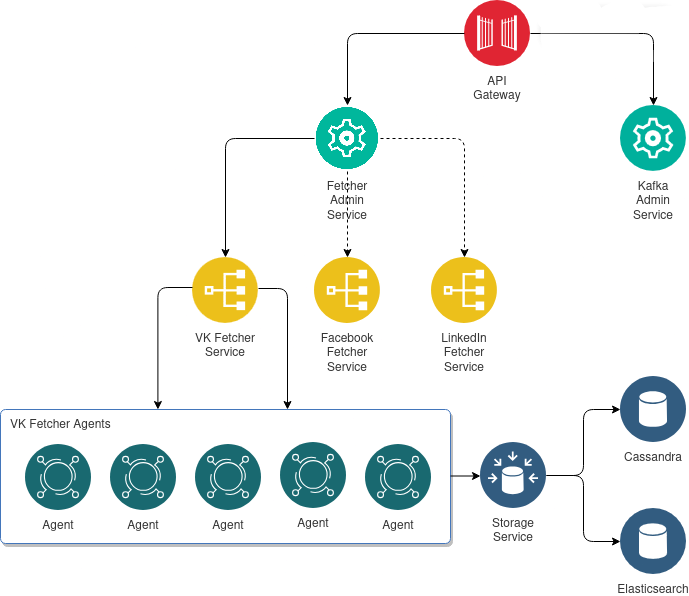
\includegraphics[scale=0.5]{architecture_diagram.png}
        \caption{Диаграма архитектуры}
    \end{figure}
    Как установлено в предыдущем разделе, проектируемая система требует одновременного обеспечения низкой задержки обработки, горизонтальной масштабируемости и устойчивости к сбоям. Реализация этих требований достигается через гибридную архитектуру, интегрирующую принципы Каппа-архитектуры с микросервисным подходом. Данный синтез формирует основу для обработки потоковых данных социальных сетей, обеспечивая баланс между производительностью, гибкостью и надёжностью.\\

    Все микросервисы системы можно отнести к нескольким слоям: \textbf{Cлой приёма данных}, \textbf{Cлой обработки}, \textbf{Cлой хранения и визуализации} и \textbf{Cлой управления и администрации}. Каждый микросервис связан с другими через топики Kafka.

    \subsection{Слой управления и администрации}
        Слой управления и администрации является главным управляющим уровнем системы. На данным слое находятся сервисы отвечающие за непосредственное управление системой.
        
        \subsubsection{Взаимодействие сервисов}
            Каждый сервис взаимодействует с другоми через Kafka. Для этого используется формат JSON. Каждая команда имеет следующую структуру:
            \begin{lstlisting}
                {
                    "target_type":
                    "content": {
                    }
                }
            \end{lstlisting}
            В поле \texttt{target\_type} устанавливает получатель тип команды, используя который, система определяет какую из структур команды использовать и обрабатывает содержимое поля \texttt{content} соответствующим образом.

            В рамках работы системы, для удобства обрыботки команд используется внутренняя структура данных, которая предварительно трансформируется в JSON и кодируется. Для создания команд используется внутренний класс-конструктор, а для трансформации - класс-обработчик. Эти классы изолированы и автоматически используются внутри специальзированной обёртка над Продюсером Kafka. Это позволяет снизить зависимости внутри системы и реализовывать взаимодействие системы без загромождения кода лишними вызовами обработчиков, что увеличивает читаемость кода и упрощает интеграцию в проект, а так же упрощает отладку. Для обратного декодирования из JSON во внутреннюю структуру используется библиотека \texttt{dacite}.

        \subsubsection{Kafka Admin Service}
            Kafka Admin Service — это сервис отвечающий за управление и администрирование Kafka. При инициализации он создаёт служебный топик и начинает обрабатывать приходящие в него команды. Основными ответственностями этого сервиса является создание и удаление топиков а так же их конфигурация, создание партиций. Через этот сервис проходит вся настройка работы Kafka.  

            Для взаимодействия с данных сервисом используется следующий формат \texttt{content}:
            \begin{lstlisting}
                "content": {
                    "command_type":
                    "id":
                    "topics_names": []
                    "topics_parameters": {
                        "name": []
                    }
                }
            \end{lstlisting}
            Где:
            \begin{itemize}
                \item \texttt{command\_type} — тип полученной команды, обозначающий целевое действие (создание топика, удаление) и влияющее на то, какие поля запроса будут использоваться.
                \item \texttt{id} — Уникальный идентификатор запроса.
                \item \texttt{topics\_names} — Список имён топиков.
                \item \texttt{topics\_parameters} — Список параметров топиков. Для каждого топика из списка имён сдесь должны быть приведены соответсвующие параметры, а именно колличество партиций и уровень реплицирования.
            \end{itemize}

        \subsubsection{Fetcher Admin Service}
            Fetcher Admin Service — это сервис отвечающие за администрацию сбора данных. Он не занимается сбором самостоятельно, а управляет сервисами по сборке данных из различных социальных сетей, например VK Fetcher Service. Основной обязанностью данного сервися является управление слоем приёма данных: добавление новых API токенов и удаление старых, управление списком обрабатываемых сообществ социальных сетей, добавление новых и удаление старых.

            Для взаимодействия с данных сервисом используется следующий формат \texttt{content}:
            \begin{lstlisting}
                "content": {
                    "command_type":
                    "id":
                    "social_media_type":
                    "groups": []
                    "APIToken":
                }   
            \end{lstlisting}
            Где:
            \begin{itemize}
                \item \texttt{command\_type} — тип полученной команды, обозначающий целевое действие (добавление API-токена, добавление сообществ в обработку) и влияющее на то, какие поля запроса будут использоваться.
                \item \texttt{id} — Уникальный идентификатор запроса.
                \item \texttt{social\_media\_type} — типо социальной сети, к которой отправляется запрос (VK, Twitter и тд)
                \item \texttt{groups} — Список групп / сообществ для добавления в обработку или удаления из неё.
                \item \texttt{APIToken} — Токен для добавления или удаления
            \end{itemize}

    \subsection{Слой приёма данных}
        Слой приёма данных — это слой системы, но котором расположены сервисы, отвечающие за сбор данных и отправку их для дальнейшей обработки в топики Kafka. На этом уровне так же реализуется обработка всех команд, с учётом особенностей системы. 

        \subsubsection{Особенности работы с VK}
            VK обладает открытым API, получить доступ к которому не составляет большого труда. Он предоставляет возможность для авторизации пользователя и собора открытой информации. Например такой информацией являются публикации в открытых группах, реакции на эти публикации и комментарии к ним. Так же с помощью Open API можно получить информацию о подписчиках сообществ, друзьях пользователей, фотографиях, видеозаписях и другой информацией, открытой пользователю. Иначе говоря VK API - это интерфейс, который позволяет получать информацию из базы данных vk.com с помощью HTTP-запросов к специальному серверу. Синтаксис запросов и тип возвращаемых ими данных строго определены на стороне самого сервиса. В ответ на запрос сервер возвращает ответ в формате JSON, что стоит учесть при выборе технологий, используемых для проектирования системы. \\

            Для отправки API-запросов используется  формат HTTP, в частности методы POST или GET. В API VK эти методы равнозначны. Запросы отправляются на адреса следующего вида:

            \texttt{https://<адрес>/method/<API-метод>?<параметры>} \\

            Где:    
            \begin{itemize}
                \item \texttt{<адрес>} — один из адресов API ВКонтакте:
                \begin{itemize}
                    \item \texttt{api.vk.com}
                    \item \texttt{api.vk.ru}
                \end{itemize}
                \item \texttt{<API-метод>} — имя раздела и API-операции для вызова, например \texttt{users.get} или \texttt{likes.add}
                \item \texttt{<параметры>} — параметры, которые передаются методу в строке запроса, например \texttt{...?v=5.199\&p1=v1}. Так же их называют query-параметрами.
            \end{itemize}

            VK API, как и API других социальных сетей, имеет ряд ограничений, которые стоит учитывать при проектировании системы:
            \begin{enumerate}
                \item Максимум 3 запроса / секунду с одного API-ключа.
                \item Для \texttt{wall.get} возвращается $\leq$ 100 последних постов в сообществе.
                \item Невозможность подписки на события в реальном времени.
                \item Невозможность получения удалённых/скрытых постов.
            \end{enumerate}

        \subsubsection{VK Fetcher Service и VK Fetchers}
            VK Fetcher Service является центральным сервисом сбора данных социальной сети VK и управляется из Fetcher Admin Service. При инициализации он отправляет запрос в Kafka Admin Service на создание служебного топика для приёма команд от Слоя управления и администрации.

            Для каждого из API-токенов VK Fetcher Service создаёт отдельный инстанс Фетчера, который в асинхронном порядке обрабатывает группы сообществ в обработке. Это нужно для того, что бы обойти ограничение на частоту запросов к API.

            После инициализации сервиса, тот разделяется на 2 асинхронных потока, один из которых обрабатывает приходящие из Слоя управления команды, а второй создаёт очередь задач. Он начинает создавать задачи на обновление данных по конкретной группе из списка сообществ на обработку, после чего складывает их в очередь. Каждый из Фетчеров в свою очередь читает эти задачи и создаёт асинхронную задачу для разпараллеливания нагрузки, после чего уходит в ожидание на $0.5$ секунды для соблюдения правил работы с API. Подобная архитектура позволяет уменьшить время простоев, одновременно регулируя и балансируя нагрузку на разные API-токены. Ещё одним приемуществом подобной архитектуры является возмжность динамически регулировать список обрабатываемых групп, а так же добавлять новые ключи, не останавливая работу сервису. Это крайне важно для регулирования больших всплесков активности и поддержания масштабируемости.

    \subsection{Слой обработки}
        Слой обработки выступает как главный рабочий слой. Он отвечает за предварительную обработку данных, их агрегацию и соверщение перобразований над ними (добавление данных, удаление ненужных и тд). Для этого используется пайплайн Kafka + Flink:             

        \subsubsection{Интеграция с Kafka}
            Kafka выступает в роли шины событий, обеспечивая надежную передачу данных между микросервисами. Сообщения группируются по топикам в зависимости от типа данных (например, посты, комментарии, внутренние команды). Для соблюдения упорядоченности данных ключи сообщений вычисляются на основе идентификатора группы, гарантируя последовательную обработку постов. 
            
            Внутри системы реализована специальная обёртка над Продюсером, которая инкапсулирует в себе предварительную обработку данных перед отправкой в топик (например преобразование в JSON). Так же перед отправкой данные кодируются в UTF-8 для обработки рускоязычного текста.
            
        \subsubsection{Интеграция с Flink}
            Apache Flink занимает центральное место в архитектуре системы, выступая в качестве высокопроизводительного движка потоковой обработки, который обеспечивает преобразование, агрегацию и анализ данных в режиме реального времени. Его интеграция в систему основана на принципах Каппа-архитектуры, что позволяет обрабатывать как текущие события, так и исторические данные через единый вычислительный конвейер, устраняя необходимость в раздельных системах для потоковой и пакетной обработки.

            Flink выполняет критически важную функцию моста между источником данных (Apache Kafka) и системами хранения/аналитики (Elasticsearch и Cassandra). Основная задача Flink в системе — обеспечить обработку каждого поста из социальной сети VK с задержкой менее 60 секунд от момента публикации до сохранения результатов. Это достигается за счет непрерывной обработки событий, преобразований данных в реальном времени и управления состоянием вычислений при длительных операций. 

            Источником данных для Flink выступают топики Apache Kafka, куда VK Fetcher Service отправляет сырые данные из социальной сети. Flink потребляет эти данные через распределенного потребителя. Ключевой особенностью является использование механизма водяных знаков (watermarks), которые позволяют Flink определять полноту данных в потоке и корректно обрабатывать события, приходящие с задержкой из-за особенностей сети или неравномерной нагрузки в социальной сети.

            Проходящие через Flink данные проходят следующие этапы преобразований:
            \begin{enumerate}
                \item \textbf{Нормализация и очистка} \\
                В первую очередь это приведение временных меток к единому формату ISO 8601, фильтрация некорректных или повреждённых записей, а так же стандартизация текстовых данных (приведение к одному регистру, нормальзация кодировки)
                \item \textbf{богащение контекстом} \\
                На этом этапе добавляются дополнительные данные. Это добавление извлечение методанных, классификация тональности с помощью ML-моделей или любые дополнительные данные, которые могут помочь на следующем этапе.
                \item \textbf{Оконная агрегация} \\
                На этом этапе выполняется расчет скользящих средних показателей (лайки, репосты) в 5-минутных окнах и обнаружение аномалий активности через статистические методы. Данный этап являтся главным для потоковой обработки.
            \end{enumerate}

            Для управления задачами в кластере Flink используется job-manager-ui, доступ к котрому пробрасывается из кластера Flink

    \subsection{Слой хранения и визуализации}
        Данный слой не реализовывался в прототипе, однако стоит отдельно упомянуть. На данном слое располагаются сервисы ответственные за хранение и подготовку данных к глубокому анализу и пакетной обработке.

        \subsubsection{Storage Service}
            Storage Service служит основным сервисом сохранения данных. Он читает полученные от Фетчеров данные, после чего сохраняет их в 2 хранилища: \textbf{Elasticsearch} (горячее хранилище) для быстрого поиска и дополнительной аналитики и \textbf{Cassandra} (холодное хранилище) для долгосрочного хранения и интеграции с глубокой, пакетной обработкой данных за большие промежутки времени. 

        \subsubsection{Elasticsearch}
            Elasticsearch интегрирован в систему как ключевой компонент для оперативной аналитики, обеспечивающий полнотекстовый поиск, агрегацию данных и визуализацию в режиме реального времени. В архитектуре системы он выполняет роль горячего хранилища и основного движка аналитики. Опционально Elasticsearch так же можно использовать для визуализации через интеграцию с Kibana. Индексы настроены с анализаторами для русскоязычного контента. Агрегации по временным гистограммам позволяют визуализировать активность пользователей. Для сохранения данных в Elasticsearch используется официальный коннектор Flink \texttt{org.apache.flink.connector\\.elasticsearch7}

            Данные поступают из Apache Flink через REST API с использованием bulk-запросов для оптимизации производительности. Для поддержания уникальности используется состовной ключ \texttt{group\_id\_post\_id}, который гарантирует уникальность записей.

        \subsubsection{Cassandra}
            CApache Cassandra в системе выполняет роль высокомасштабируемоего распределенного хранилища для долгосрочного хранения больших объемов данных. В архитектуре системы она выполняет функции основного хранилища для сырых данных и агрегированных показателей, платформы для исторического анализа данных за длительные периоды и системы резервного копирования. Схема таблиц может быть оптимизирована для высокой скорости записи, а горизонтальная масштабируемость достигнута без изменения архитектуры добавлением новых нод.  

            Ключевое пространство social\_media может быть организовано с учетом специфики социальных данных. Это достигается за счёт стратегии репликации: NetworkTopology-Strategy обеспечивает копирование данных между дата-центрами (например, 3 копии в основном DC, 2 - в резервном), а так же проектированием таблиц с опорой на особенности данных. Основные таблицы:
            \begin{itemize}
                \item \textbf{raw\_posts} — Хранит исходные данные постов с партиционированием по ID группы
                \item \textbf{daily\_aggregates} — Содержит предварительно агрегированные дневные метрики (количество постов, средние лайки/комментарии)
                \item \textbf{backups} — Архивные копии данных из Elasticsearch
            \end{itemize}

            Для повышения безопасности и отказоустойчивости, данные раз в несколько дней копируются из Elasticsearch и распределяются по дата-центрам, каждая копия содержит метку времени и идентификатор источника.

    \subsection{K8S}
        Для упрощения запуска системы, её развёртывания и масштабирования, для каждого сервиса был написан Dockerfile и yml-файл, что позволяет запустить систему в K8S. Это значительно упрощает управление системой, открывает доступ к реализации автоматического масштабирования любого сервиса и оркестризации. Так же это упрощает интеграцию с Flink и Kafka, за счёт использования уже готовых Docker-образов. 
    
    \subsection{Соответствие требованиям}
        Соответствие требованиям подтверждено замерами задержки в обработке сообществ ВК. Замерялось время обработки всех сообществ из списка обработки.  Для удобства анализа данные изображены на графике. 
        \begin{figure}
            \centering
            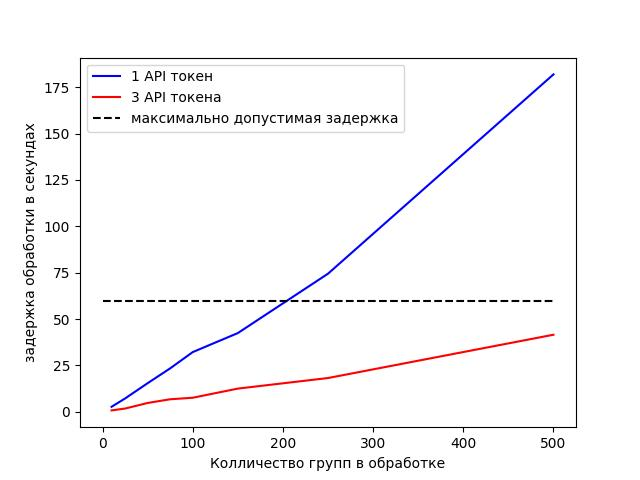
\includegraphics[scale=0.7]{benchmark.jpeg}
            \caption{График задержки обработки}
        \end{figure}

        Как можно заметить главным узким местом системы, как и предполагалось является отправка и обработка запросов VK. Однако при масштабировании колличества API-токенов, система автоматически использует новые ресурсы и задержка значительно снижается. Таким образом для обработки 500 групп достаточно 3-х API-токенов, а для обработки 10000 сообществ с задержкой менее минуты, достаточно 50 токенов.

        Так же были сняты замеры времени обработки одного сообщества. Для прохождения всего пайплайна сообществом, системе необхадимо $0.4$ секунды.
        
    \subsection{Исследование системы на предмет улучшений и ускорения}
        Для разработанной системы был проведён анализ узких мест и предложены варианты для их улучшения и оптимизации:
        \begin{enumerate}
            \item Одним из самых узких мест в системе оказалась ситема фетчинга данных социальных сетей. Для решения этой предлагаются следующие улучшения: автоматическое удаление недоступных и закрытых сообществ, оптимизация обновления данных группы, основываясь на частоте публикаций в сообществе. Нарпимер сообщество которое публикует новости раз в сутки менее целесообразно опрашивать каждую минуту, в отличии от сообществ, публикующих данные каждые 10 минут. Динамически настраивая подобные параметры, можно добиться ускорения в несколько раз. Однако всё ещё нужно оставить возможность отключения этой функции для конкретных сообществ, для сообществ, требующих максимально высокой точности и низкой задержки.
            \item Ускорение Flink-Обработки возможно достичь с помощью предварительной агрегации данных и оптимизации состояний, а так же векторизации обработки. таким образом можно будет достичь сокращение времени обработки окон на $25-35\%$ 
            \item Оптимизация Доступа к Данным может стать необхадима при увеличении колличества обрабатываемых данных. Для Elasticsearch этих оптимизаций можно достичь за счёт гибридного кэша в Radis (самые активыне сообщества и пользователи) и прекомпиляции шаблонов запросов.
            \item В случае необхадимости оптимизации Kafka, например при росте задержек при малом размере сообщений, можно воспользоваться сжатием данных, перед отправкой в Kafka, например при помощи настройки Kafka (compression\_type="snappy") или использованием zstd
        \end{enumerate}
        
\newpage
 %% Описание практической части
    \section{Заключение}
\label{sec:Chapter5} \index{Chapter5}
    Настоящее исследование посвящено проектированию, разработке и реализации прототипа системы потоковой обработки данных социальных сетей, ориентированной на анализ пользовательского контента в режиме реального времени. В ходе работы достигнуты следующие ключевые результаты:

    \begin{enumerate}
        \item Предложена \textbf{гибридная архитектура}, интегрирующая принципы \textbf{Kappa-архи-тектуры} (единый поток событий, репроцессинг данных) с \textbf{микросервисным подходом}. Это позволило ликвидировать дублирование логики обработки и обеспечить модульность и независимое масштабирование компонентов.
        
        \item Разработан \textbf{механизм сбора данных} VK на базе асинхронного фреймворка \textbf{vkbottle}, обеспечивающий:
        \begin{itemize}
            \item Обход ограничений rate limit (3 запроса/секунду) через динамическое распределение задач по API-токенам
            \item Минимизацию задержек за счёт оптимизированной очереди задач
            \item Гибкое управление источниками через Fetcher Admin Service
        \end{itemize}
        
        \item Реализован \textbf{прототип конвейера обработки} на базе \textbf{Apache Kafka} (шина событий с "ровно один раз" семантикой) удовлетворяющий требованию задержки < 60 секунд. Исследована возможность подключения к конвееру Apache Flink для потоковой обработки и анализа данных
        
        Исследована и разработана архитектура, учитывающая \textbf{двухуровневую систему хранения}:
        \begin{itemize}
            \item \textbf{Elasticsearch} для оперативного поиска и визуализации
            \item \textbf{Cassandra} для долгосрочного хранения и интеграции с пакетной аналитикой
        \end{itemize}
    \end{enumerate}

    \subsection{Практическая значимость} 
        Практическая значимость работы заключается в создании универсальной платформы для маркетингового анализа (тренды, репутация брендов), социологических исследований (динамика настроений) и кризисного мониторинга (детекция аномалий)

    \subsection{Перспективные направления развития}:
        Работа имеет перспективные направления для развития в области Обработки данных. В качестве направлений развития выделены следующие варианты:
        \begin{itemize}
            \item Добавление поддержка Telegram/Twitter через модули Fetcher Admin Service
            \item Полноценная интеграция Apache Flink для потоковой обработки детализированных
            \item Реализация хранилищ данных на основе исследованных вариантов.
            \item Исследование использования шардирования в Cassandra
            \item Внедрение ML-пайплайнов для классификации контента
            \item Оптимизация Flink-операторов для снижения задержки до 10-20 секунд
            \item Исследование методов сжатия данных в Kafka/Cassandra
        \end{itemize}

    Таким образом, разработанное решение подтверждает эффективность гибридного подхода для задач потоковой обработки Big Data, сочетая оперативность Kappa-архитектуры с гибкостью микросервисов, и открывает пути для дальнейшей оптимизации в условиях экспоненциального роста социальных данных.

\newpage
 %% Заключение

    %% НЕ ТРОГАЙТЕ!!!
    \nocite{*}
    \bibliography{references}

    %% в зависимости от надобности подключаем раздел "Приложение"
    % \newpage
    % \input{Appendix.tex}
\end{document}
